\documentclass[aspectratio=169,13pt,t] {beamer}
%
% Choose how your presentation looks.
%
% For more themes, color themes and font themes, see:
% http://deic.uab.es/~iblanes/beamer_gallery/index_by_theme.html
%
\mode<presentation>
{
  \usetheme{Madrid}      % or try Darmstadt, Madrid, Warsaw, ...
  \usecolortheme{beaver} % or try albatross, beaver, crane, ...
  \usefonttheme{serif}  % or try serif, structurebold, ...
%  \setbeamertemplate{navigation symbols}{}
  \setbeamertemplate{caption}[numbered]
  \setbeamertemplate{items}[default]
}

\usepackage[,UTF8,linespread=1.2]{ctex}
\usepackage{wrapfig}
\usepackage{caption}
\captionsetup[figure]{name=图,labelsep=period}
\usepackage[,most]{tcolorbox}
\usepackage{picinpar}
\usetikzlibrary{intersections,calc}

\usepackage{xcolor}
\definecolor{xy_blue}{cmyk}{0.6,0.35,0.0,0.4}
\definecolor{xy_orange}{cmyk}{0.0,0.7,1.0,0.0}
\definecolor{xy_green}{cmyk}{0.2,0.0,1.0,0.15}
\xdefinecolor{xy_gold}{RGB}{135,103,79}
\xdefinecolor{xy2_gold}{cmyk}{0,0.35,0.75,0.05}


\setbeamercolor{section number projected}{fg=red,bg=red!20}%控制球的颜色
\setbeamercolor{subsection number projected}{fg=blue,bg=blue!40}
\setbeamercolor{item}{fg=xy_gold} %设置列表项颜色

\usepackage{amsthm}
\newtheorem{peroration}{结论：}
\newtheorem{exploration}{探究：}
\newtheorem{prooft}{证明：}
\newtheorem{question}{问题}
\newtheorem*{solve}{解:}
\newtheorem{instance}{例}   % 解：独立计数器
\BeforeBeginEnvironment{peroration}{%
	\setbeamercolor{block title}{bg=xy_green,fg=white}
	\setbeamercolor{block body}{bg=xy_green!10}
}
\AfterEndEnvironment{peroration}{
	\setbeamercolor{block title}{bg=xy_blue,fg=white}
	\setbeamercolor{block body}{bg=xy_blue!10}
}
\BeforeBeginEnvironment{exploration}{%
	\setbeamercolor{block title}{bg=xy_orange,fg=white}
	\setbeamercolor{block body}{bg=xy_orange!10}
}
\AfterEndEnvironment{peroration}{
	\setbeamercolor{block title}{bg=xy_blue,fg=white}
	\setbeamercolor{block body}{bg=xy_blue!10}
}
\BeforeBeginEnvironment{solution}{%
	\setbeamercolor{block title}{bg=xy_green,fg=white}
	\setbeamercolor{block body}{bg=xy_green!10}
}
\AfterEndEnvironment{solution}{
	\setbeamercolor{block title}{bg=xy_green,fg=white}
	\setbeamercolor{block body}{bg=xy_green!10}
}
\BeforeBeginEnvironment{prooft}{%
	\setbeamercolor{block title}{bg=xy_green,fg=white}
	\setbeamercolor{block body}{bg=xy_green!10}
}
\AfterEndEnvironment{prooft}{
	\setbeamercolor{block title}{bg=xy_green,fg=white}
	\setbeamercolor{block body}{bg=xy_green!10}
}
\BeforeBeginEnvironment{question}{%
	\setbeamercolor{block title}{bg=xy_orange,fg=white}
	\setbeamercolor{block body}{bg=xy_orange!10}
}
\AfterEndEnvironment{question}{
	\setbeamercolor{block title}{bg=xy_green,fg=white}
	\setbeamercolor{block body}{bg=xy_green!10}
}
\BeforeBeginEnvironment{solve}{%解：
	\begingroup
	\setbeamercolor{block title}{bg=xy_orange!60,fg=white}
	\setbeamercolor{block body}{bg=xy_orange!10}
}
\AfterEndEnvironment{solve}{%解：
	\endgroup
}

\setbeamercolor{prooft}{fg=red, bg=green!10}       % 标题颜色
\setbeamercolor{prooft body}{fg=red, bg=red!5}  % 内容块背景
\setbeamerfont{prooft head}{series=\bfseries}       % 标题字体
\setbeamerfont{question body}{shape=\upshape}         % 内容字体
\renewcommand{\thefigure}{\arabic{figure}}

\newtcolorbox{summarybox}[1][]{
	colback=purple!10,
	colframe=purple!70!black,
	fonttitle=\bfseries,
	title=#1,
	arc=1mm,
	boxrule=0pt,drop shadow,
	left=2mm, right=2mm, top=2mm, bottom=2mm,
}
\newtcolorbox{summarybox-answer}{
%	width=0.9\textwidth,
	colback=white,
	blanker,
	borderline west={2pt}{2pt}{cyan},
	left=2mm, right=2mm, top=2mm, bottom=2mm,
	}
\title[3.2.1 单调性与最大(小)值]{3.2.1 单调性与最大(小)值}
\subtitle{增函数与减函数、单调区间、最大值与最小值}
\author[好好学习，努力向上]{}
\institute{}
\date{2026.10.13}
%\setbeamertemplate{theorems}[numbered]
\theoremstyle{definition}
\newtheorem{exam}{例}
\AtBeginSection[]
{
  \begin{frame}<beamer>
    \frametitle{本节主要内容}
    \tableofcontents[currentsection,currentsubsection]
  \end{frame}
}

\AtBeginDocument{
	\setlength{\abovedisplayskip}{3pt}
	\setlength{\belowdisplayskip}{3pt}
	\setbeamertemplate{theorems}[numbered]
}

\usepackage{pgfplots}
\pgfplotsset{compat=1.18}
\usetikzlibrary{arrows.meta}

\begin{document}
\begin{frame}{}
	\titlepage
\end{frame}

\begin{frame}{内容概览}
	\tableofcontents
\end{frame}

\section{单调性的概念}

\begin{frame}{观察：二次函数 \(f(x)=x^2\) 的图象}
	在初中，我们利用函数图象研究过函数值随自变量增大而增大（或减小）的性质，这一性质叫做函数的\textbf{单调性}.
	\begin{columns}[t]
		\column{0.40\textwidth}\hspace{2em}
		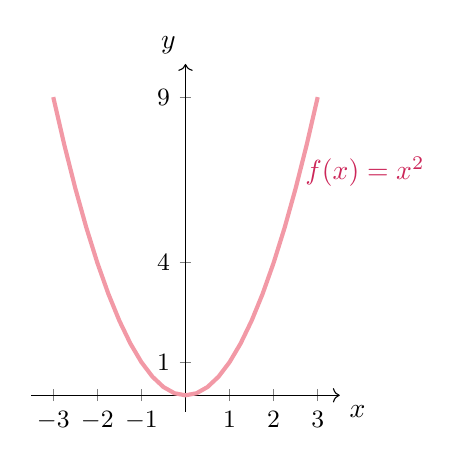
\begin{tikzpicture}[baseline=3cm]
			\begin{axis}[
				clip=false,
				width=5.5cm, height=6cm,
				xmin=-3.5, xmax=3.5,
				ymin=-0.5, ymax=10,
				xtick={-3,-2,-1,0,1,2,3},
				ytick={1,4,9},
				axis lines=middle,
				axis line style={->},
				xlabel={$x$}, ylabel={$y$},
				xlabel style={below right},
				ylabel style={above left},
				tick label style={font=\small},
			]
			\addplot[color=pink!80!purple, line width=1.5pt, domain=-3:3] {x^2};
			\node[above right, pink!20!purple] at (2.5, 6) {$f(x)=x^2$};
			\end{axis}
		\end{tikzpicture}

	
		\column{0.6\textwidth}
		\begin{minipage}{\textwidth}
		\begin{summarybox-answer}
			图象在 \(y\) 轴左侧从左到右\textbf{下降}：当 \(x\leqslant 0\) 时，\(y\) 随 \(x\) 增大而减小.\\[4pt]
			图象在 \(y\) 轴右侧从左到右\textbf{上升}：当 \(x\geqslant 0\) 时，\(y\) 随 \(x\) 增大而增大.
		\end{summarybox-answer}
	\end{minipage}
	\end{columns}
\end{frame}

\begin{frame}{增函数与减函数的定义}
	一般地，设函数 \(f(x)\) 的定义域为 \(D\)，区间 \(I\subseteq D\)：
	\begin{summarybox}[单调递增]
	如果 \(\forall x_1,x_2\in I\)，当 \(x_1<x_2\) 时，都有 \(f(x_1)<f(x_2)\)，那么称函数 \(f(x)\) 在区间 \(I\) 上\textbf{单调递增}.
	\end{summarybox}
	\begin{summarybox}[单调递减]
	如果 \(\forall x_1,x_2\in I\)，当 \(x_1<x_2\) 时，都有 \(f(x_1)>f(x_2)\)，那么称函数 \(f(x)\) 在区间 \(I\) 上\textbf{单调递减}.
	\end{summarybox}
	\vspace{0.5em}
	\begin{summarybox-answer}
	特别地，当函数在它的定义域上单调递增时，称它是\textbf{增函数}；单调递减时，称它是\textbf{减函数}. 区间 \(I\) 叫做函数的\textbf{单调区间}.
	\end{summarybox-answer}
\end{frame}

\begin{frame}{图象直观：上升与下降}
	\begin{columns}
		\column{0.5\textwidth}
		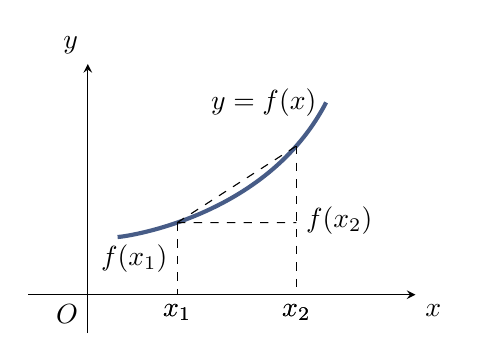
\begin{tikzpicture}[baseline={(0,0)}]
			\begin{axis}[
				clip=false,
				width=6.5cm, height=5cm,
				xmin=-1, xmax=5.5, ymin=-1, ymax=6,
				xtick=\empty, ytick=\empty,
				axis lines=middle, axis line style={->},
				xlabel={$x$}, ylabel={$y$},
				xlabel style={below right}, ylabel style={above left},
				>=stealth,
			]
			\draw[name path =curve,line width=1.5pt,color=xy_blue] 
				(0.5,1.5) .. controls (0.6,1.5) and (3.0,2) .. (4,5);
			\path [name path =a_1] (1.5,0) -- (1.5,5);
			\path [name path = b_1] (3.5,0) -- (3.5,5);
			\path [name intersections={of =curve and a_1,by=a}]  ;
			\path [name intersections={of =curve and b_1,by=b}]  ;
			\draw[dashed] (a) -- (a |- 0,0)node[below]{$x_1$};
			\draw[dashed] (b) -- (b |- 0,0)node[below]{$x_2$};
			\draw [dashed] (a) -|(a -| b) (a) -- (b);
			\node[below] at (1.5,0) {$x_1$};
			\node[below] at (3.5,0) {$x_2$};
			\node[left] at ($(a)!0.5!(a |- 0,0)$) {$f(x_1)$};
			\node[right] at ($(b)!0.5!(b |- 0,0)$) {$f(x_2)$};
			\node[left] at (4,5) {$y=f(x)$};
			\node[below left] at (0,0) {$O$};
			\end{axis}
		\end{tikzpicture}
		
		\centering\small 单调递增（上升）
		\captionof{figure}{}
		
		\column{0.5\textwidth}
		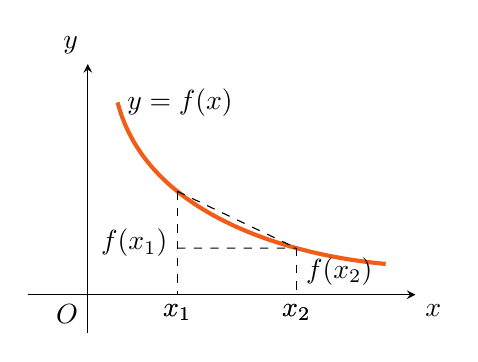
\begin{tikzpicture}[baseline={(0,0)}]
			\begin{axis}[
				clip=false,
				width=6.5cm, height=5cm,
				xmin=-1, xmax=5.5, ymin=-1, ymax=6,
				xtick=\empty, ytick=\empty,
				axis lines=middle, axis line style={->},
				xlabel={$x$}, ylabel={$y$},
				xlabel style={below right},
				ylabel style={above left},
				>=stealth,
			]
			\draw[name path=curve,line width=1.5pt,color=xy_orange] (0.5,5) .. controls (1,2) and (3.5,1) .. (5,0.8);
			\path [name path =a_1] (1.5,0) -- (1.5,5);
			\path [name path = b_1] (3.5,0) -- (3.5,5);
			\path [name intersections={of =curve and a_1,by=a}]  ;
			\path [name intersections={of =curve and b_1,by=b}]  ;
			\draw[dashed] (a) -- (a |- 0,0)node[below]{$x_1$};
			\draw[dashed] (b) -- (b |- 0,0)node[below]{$x_2$};
			\draw [dashed] (a |- b) -- (b) (a) -- (b);
			\node[below] at (1.5,0) {$x_1$};
			\node[below] at (3.5,0) {$x_2$};
			\node[left] at ($(a)!0.5!(a |- 0,0)$) {$f(x_1)$};
			\node[right] at ($(b)!0.5!(b |- 0,0)$) {$f(x_2)$};
			\node[right] at (0.5,5) {$y=f(x)$};
			\node[below left] at (0,0) {$O$};
			\end{axis}
		\end{tikzpicture}
	
		\centering\small 单调递减（下降）	
		\captionof{figure}{}
	\end{columns}
\end{frame}

\section{单调性的证明}

\begin{frame}{例1：研究 \(f(x)=kx+b\,(k\neq 0)\) 的单调性}
	\begin{exam}
	根据定义，研究函数 \(f(x)=kx+b\,(k\neq 0)\) 的单调性.
	\end{exam}
	\pause
	\begin{solve}
	函数 \(f(x)=kx+b\) 的定义域是 \(\mathbf{R}\). 任取 \(x_1,x_2\in\mathbf{R}\)，且 \(x_1<x_2\)，则
	\[
		f(x_1)-f(x_2)=(kx_1+b)-(kx_2+b)=k(x_1-x_2).
	\]
	由 \(x_1<x_2\)，得 \(x_1-x_2<0\).
	\end{solve}
\end{frame}

\begin{frame}{例1（续）：分类讨论 \(k\) 的符号}
	\begin{solve}
	① 当 \(k>0\) 时，\(k(x_1-x_2)<0\)，于是 \(f(x_1)-f(x_2)<0\)，即 \(f(x_1)<f(x_2)\).\\
	\quad 这时 \(f(x)=kx+b\) 是\textbf{增函数}.
	\end{solve}
	\vspace{0.5em}
	\pause
	\begin{solve}
	② 当 \(k<0\) 时，\(k(x_1-x_2)>0\)，于是 \(f(x_1)-f(x_2)>0\)，即 \(f(x_1)>f(x_2)\).\\
	\quad 这时 \(f(x)=kx+b\) 是\textbf{减函数}.
	\end{solve}
	\vspace{0.5em}
	\begin{summarybox-answer}
	\textbf{证明四步}：取值（设 \(x_1<x_2\)）\(\to\) 作差 \(f(x_1)-f(x_2)\)\(\to\) 变形（因式分解）\(\to\) 定号（判断与 \(0\) 的大小）.
	\end{summarybox-answer}
\end{frame}

\begin{frame}{例3：证明 \(y=x+\dfrac{1}{x}\) 在 \((1,+\infty)\) 上单调递增}
	\begin{exam}
	根据定义证明函数 \(y=x+\dfrac{1}{x}\) 在区间 \((1,+\infty)\) 上单调递增.
	\end{exam}
	\pause
	\begin{prooft}
	任取 \(x_1,x_2\in(1,+\infty)\)，且 \(x_1<x_2\)，有
	\[
		y_1-y_2=\Bigl(x_1+\frac{1}{x_1}\Bigr)-\Bigl(x_2+\frac{1}{x_2}\Bigr)
		=(x_1-x_2)+\frac{x_2-x_1}{x_1x_2}
		=\frac{x_1-x_2}{x_1x_2}(x_1x_2-1).
	\]
	\end{prooft}
\end{frame}

\begin{frame}{例3（续）：定号}
	\begin{prooft}
	由 \(x_1,x_2\in(1,+\infty)\)，得 \(x_1>1,\ x_2>1\)，所以 \(x_1x_2>1\)，即 \(x_1x_2-1>0\).\\
	又由 \(x_1<x_2\)，得 \(x_1-x_2<0\). 于是
	\[
		\frac{x_1-x_2}{x_1x_2}(x_1x_2-1)<0,\quad\text{即 } y_1<y_2.
	\]
	所以，函数 \(y=x+\dfrac{1}{x}\) 在区间 \((1,+\infty)\) 上\textbf{单调递增}.
	\end{prooft}
	\vspace{0.5em}
	\begin{summarybox-answer}
	\textbf{关键}：作差后通过通分、因式分解，把差化成几个因式乘积的形式，再逐一判断符号.
	\end{summarybox-answer}
\end{frame}

\begin{frame}{小结}
	单调性概念：
	\begin{enumerate}[(1)]
		\item<2-> 单调递增
		\item<3-> 单调递减
	\end{enumerate}
\end{frame}

\begin{frame}{布置作业}
	P79 练习 ：1，2，3，4
	
	P85---86 习题3.2： 1，2，4
\end{frame}

\section{最大(小)值}

\begin{frame}{最大值与最小值的定义}
	观察 \(f(x)=x^2\) 的图象，它有一个最低点 \((0,0)\)，即 \(\forall x\in\mathbf{R}\)，都有 \(f(x)\geqslant f(0)\).
	\begin{summarybox}[最大值]
	设函数 \(y=f(x)\) 的定义域为 \(D\)，如果存在实数 \(M\) 满足：\\
	(1) \(\forall x\in D\)，都有 \(f(x)\leqslant M\)；\quad (2) \(\exists x_0\in D\)，使得 \(f(x_0)=M\).\\
	那么称 \(M\) 是函数 \(y=f(x)\) 的\textbf{最大值}.
	\end{summarybox}
	\begin{summarybox-answer}
	\textbf{最小值}：把上述定义中的 \(f(x)\leqslant M\) 改为 \(f(x)\geqslant M\)，其余条件不变，即得最小值的定义.
	\end{summarybox-answer}
\end{frame}

\begin{frame}{例4：烟花爆裂的最佳时刻}
	\begin{exam}
	“菊花”烟花冲出后距地面高度 \(h(t)=-4.9t^2+14.7t+18\)（单位：m）. 求烟花冲出后何时是爆裂的最佳时刻，这时距地面高度约为多少（精确到 \(1\,\mathrm{m}\)）？
	\end{exam}
	\pause
	\begin{solve}
	二次函数 \(h(t)=-4.9t^2+14.7t+18\) 开口向下，顶点即最高点.
	\[
		t=-\frac{14.7}{2\times(-4.9)}=1.5\ (\mathrm{s}),\qquad
		h=\frac{4\times(-4.9)\times18-14.7^2}{4\times(-4.9)}\approx 29\ (\mathrm{m}).
	\]
	\end{solve}
\end{frame}

\begin{frame}{例4（图）：高度随时间变化}
	\begin{columns}
		\column{0.58\textwidth}
		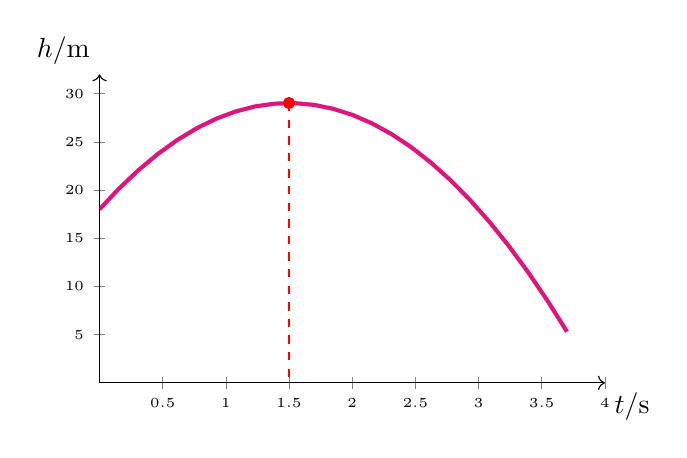
\begin{tikzpicture}
			\begin{axis}[
				width=8cm, height=5.5cm,
				xmin=0, xmax=4, ymin=0, ymax=32,
				xtick={0,0.5,1,1.5,2,2.5,3,3.5,4},
				ytick={5,10,15,20,25,30},
				axis lines=middle, axis line style={->},
				xlabel={$t$/s}, ylabel={$h$/m},
				xlabel style={below right}, ylabel style={above left},
				tick label style={font=\tiny},
			]
			\addplot[color=magenta!70!purple, line width=1.5pt, domain=0:3.7] {-4.9*x^2+14.7*x+18};
			\addplot[only marks, mark=*, mark size=2pt, color=red] coordinates {(1.5,29.025)};
			\draw[dashed, red] (1.5,29.025) -- (1.5,0);
			\end{axis}
		\end{tikzpicture}
		\column{0.38\textwidth}
		\vspace{2em}
		\begin{summarybox-answer}
		烟花冲出后 \(1.5\,\mathrm{s}\) 是爆裂的最佳时刻，这时距地面高度约为 \(29\,\mathrm{m}\).
		\end{summarybox-answer}
	\end{columns}
\end{frame}

\begin{frame}{例5：求 \(f(x)=\dfrac{2}{x-1}\)，\(x\in[2,6]\) 的最值}
	\begin{exam}
	已知函数 \(f(x)=\dfrac{2}{x-1}\)（\(x\in[2,6]\)），求函数的最大值和最小值.
	\end{exam}
	\pause
	\begin{solve}
	任取 \(x_1,x_2\in[2,6]\)，且 \(x_1<x_2\)，则
	\[
		f(x_1)-f(x_2)=\frac{2}{x_1-1}-\frac{2}{x_2-1}
		=\frac{2(x_2-x_1)}{(x_1-1)(x_2-1)}.
	\]
	由 \(2\leqslant x_1<x_2\leqslant6\)，得 \(x_2-x_1>0,\ (x_1-1)(x_2-1)>0\)，于是 \(f(x_1)-f(x_2)>0\).
	\end{solve}
\end{frame}

\begin{frame}{例5（图）：端点处取得最值}
	\begin{columns}
		\column{0.55\textwidth}
		\begin{tikzpicture}
			\begin{axis}[
				width=7.5cm, height=5.5cm,
				xmin=0, xmax=7, ymin=0, ymax=2.5,
				xtick={1,2,3,4,5,6},
				ytick={0.4,0.5,1,1.5,2},
				axis lines=middle, axis line style={->},
				xlabel={$x$}, ylabel={$y$},
				xlabel style={below right}, ylabel style={above left},
				tick label style={font=\tiny},
			]
			\addplot[color=cyan!70!blue, line width=1.5pt, domain=2:6] {2/(x-1)};
			\addplot[only marks, mark=*, mark size=2pt, color=red] coordinates {(2,2) (6,0.4)};
			\end{axis}
		\end{tikzpicture}
		\column{0.42\textwidth}
		\vspace{1em}
		\begin{summarybox-answer}
		所以 \(f(x)=\dfrac{2}{x-1}\) 在 \([2,6]\) 上\textbf{单调递减}.\\[4pt]
		在 \(x=2\) 时取得最大值 \(2\)；在 \(x=6\) 时取得最小值 \(0.4\).
		\end{summarybox-answer}
	\end{columns}
\end{frame}

\section{课堂练习}

\begin{frame}{练习 1：证明 \(f(x)=3x+2\) 是增函数}
	\begin{question}
	根据定义证明函数 \(f(x)=3x+2\) 是增函数.
	\end{question}
	\pause
	\begin{solve}
	任取 \(x_1,x_2\in\mathbf{R}\)，且 \(x_1<x_2\)，则
	\[
		f(x_1)-f(x_2)=(3x_1+2)-(3x_2+2)=3(x_1-x_2)<0,
	\]
	即 \(f(x_1)<f(x_2)\). 所以 \(f(x)=3x+2\) 是\textbf{增函数}.
	\end{solve}
\end{frame}

\begin{frame}{练习 2：求 \(f(x)=\dfrac{1}{x}\) 在 \([2,6]\) 上的最值}
	\begin{question}
	已知函数 \(f(x)=\dfrac{1}{x}\)，求函数在区间 \([2,6]\) 上的最大值和最小值.
	\end{question}
	\pause
	\begin{solve}
	\(f(x)=\dfrac{1}{x}\) 在 \([2,6]\) 上单调递减（作差仿例5可证）.\\
	故在 \(x=2\) 时取最大值 \(\dfrac{1}{2}\)；在 \(x=6\) 时取最小值 \(\dfrac{1}{6}\).
	\end{solve}
\end{frame}

\begin{frame}{布置作业}
	\begin{summarybox}[课后作业]
		\begin{enumerate}
			\item 教材 P85 习题 3.2：3（1）（2），4，5
			\item 证明：函数 \(f(x)=x^2+1\) 在 \((0,+\infty)\) 上单调递增.
			\item 预习：函数的奇偶性
		\end{enumerate}
	\end{summarybox}
\end{frame}

\end{document}
